%sri

\section{Experiments}

\subsection{Index Tasks}

\paragraph{Growth of memory as execution proceeds}
\paragraph{Performance overhead as execution proceeds}



\begin{center}
 \begin{tabular}{||c c c c||} 
 \hline
 Number of Iterations (1000 tasks/index launch, seconds) & Time Without Resilience Without lg:resilient & Time Without Resilienct With lg:resilient & Time With Resilience without lg:resilient \\ [0.25ex] 
 \hline\hline
100 &  7.2 & 6.6 & 23.6\\ 
 \hline
200 &  13.8 & 13.3 & 46.3\\ 
 \hline
400 &  26.1 & 26.5 & 94.4\\ 
 \hline
800 &  55 & 53 & 186.8\\ 
 \hline
1000 &  65 & 66 & 239.9\\ [1ex] 
 \hline
\end{tabular}
\end{center}

\begin{figure}
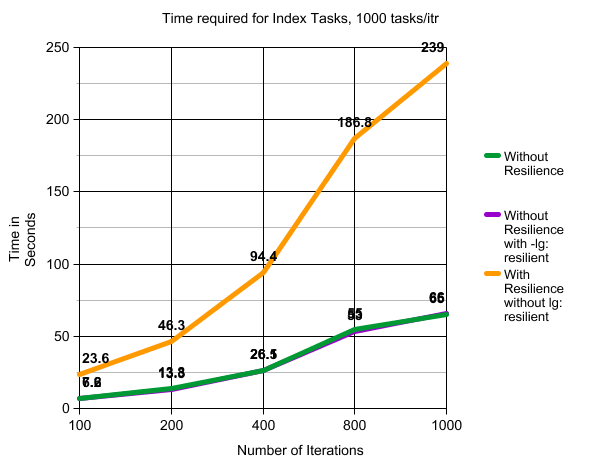
\includegraphics[width=\textwidth]{images/index_tasks_time.png}
\caption{Total time taken by 02\_index\_tasks.}
\end{figure}


\begin{figure}
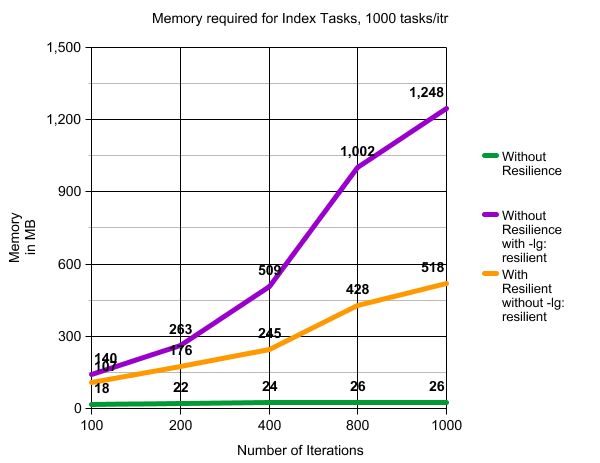
\includegraphics[width=\textwidth]{images/index_tasks_memory.png}
\caption{Total Memory footprint by 02\_index\_tasks.}
\end{figure}


\begin{center}
 \begin{tabular}{||c c c c||} 
 \hline
 Number of Iterations (1000 tasks/index launch, MB) & Memory\% Without Resilience Without lg:resilient & Memory\% Without Resilienct With lg:resilient & Memory\% With Resilience without lg:resilient \\ [0.25ex] 
 \hline\hline
100 &  18 & 140 & 107 \\ 
 \hline
200 &  22 & 263 & 176 \\ 
 \hline
400 &  24 & 509 & 245 \\ 
 \hline
800 &  26 & 1002 & 428\\ 
 \hline
1000 & 26 & 1248 & 518\\ [1ex] 
 \hline
\end{tabular}
\end{center}




\subsection{Stencil}



\subsection{local recover vs global recovery}

\subsection{compute/comm vs no-failure/single failure/multi-failure}

\subsection{S3D, Pennant, Stencil, Circuit}

\subsection{Some Interesting Task Graphs for Recovery}


